\documentclass[tikz,border=2pt]{standalone}
\usepackage{pgfplots}
\usetikzlibrary{shapes.geometric, intersections, calc}
\pgfplotsset{compat=1.7}

\begin{document}
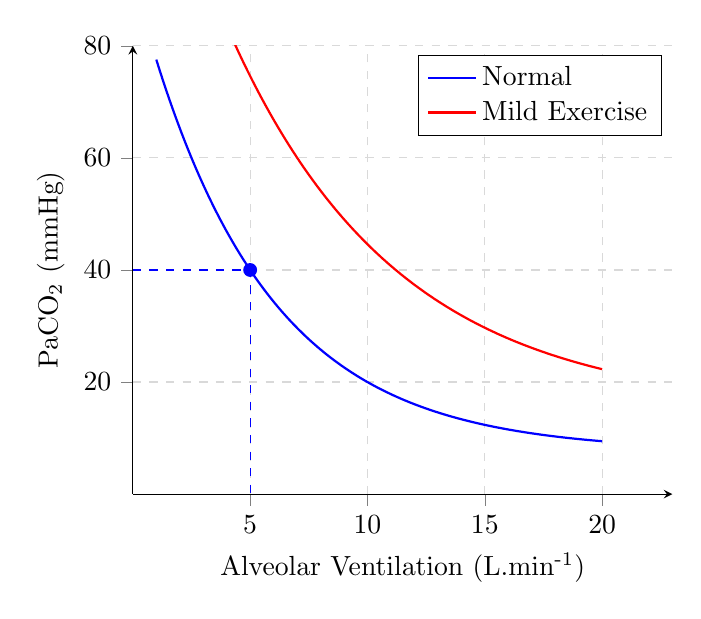
\begin{tikzpicture}


    \begin{axis}[
        axis x line=middle,
        axis y line=middle,
        grid = major,
        grid style={dashed, gray!30},
    	  x label style={at={(axis description cs:0.5,-0.1)},anchor=north},
	  y label style={at={(axis description cs:-0.1,.5)},rotate=90,anchor=south},
        xmin=0,
        xmax= 23,
        ymin= 0,
        ymax= 80,
	 ylabel near ticks,
	xlabel near ticks,
        xlabel=Alveolar Ventilation (L.min\textsuperscript{-1}),
        ylabel=PaCO\textsubscript{2} (mmHg),
        tick align=outside,
        enlargelimits=false,
legend cell align={left}]

	\addplot[domain=1:20, blue, thick,samples=500] {7.63932 + 84.72136*e^(-0.1924847*x)};
\addlegendentry{Normal};

	\addplot[domain=1:20, red, thick,samples=500] {15 + 120*e^(-0.14*x)};
\addlegendentry{Mild Exercise};

\draw[thin,dashed,blue] (axis cs: 0,40) -- (axis cs: 5,40) node[circle,fill=blue, thin, dashed,inner sep=0pt,minimum size=5pt]{} -- (axis cs: 5,0);

\end{axis}

\end{tikzpicture} 
\end{document}